%=======================================================
% CHAPTER 2: GEOMETRY OF NUMBERS
%=======================================================

\begin{frame}[plain]
  \begin{center}\bfseries\centering
    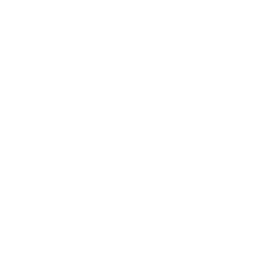
\includegraphics[scale=1]{assets/branding/opa0}
    \vspace{-5.75cm}\\
    {\adjustbox{scale=1.75}{\color{TealDarkCyan}\;III.\;Geometry of Numbers}}
    \vspace{.25cm}
    \begin{minipage}{.78\textwidth}
      \scriptsize\color{Ink}
      \textbf{Big picture.}\; Geometry proves that short structure must exist before algorithms try to find it.\\[.2cm]
      \textbf{Details to watch.}\; successive minima, Minkowski bounds, Gaussian heuristic, and packing density.
    \end{minipage}
    {\ }\vspace{2.1cm}\\
    \bigskip
  \end{center}
\end{frame}

\begin{frame}[shrink=5]{\textbf{III. Geometry of Numbers}}{Shortest Vector}
\defbox[First minimum]{
The first successive minimum of $\Lat$ is
\[
  \lambda_1(\Lat)=\min\set{\norm{v}:v\in\Lat\setdiff\{0\}}.
\]
Any nonzero $v\in\Lat$ with $\norm v=\lambda_1(\Lat)$ is a shortest vector.
}
\begin{columns}[T,onlytextwidth]
\begin{column}{.52\textwidth}
\begin{itemize}
  \item $\lambda_1$ is geometric: it does not depend on the basis.
  \item It is hard to read from a badly skewed basis.
  \item Cryptography uses the gap between basis description and geometric search.
\end{itemize}
\textbf{Example.}\; For $\Lat=2\Z\times5\Z$, the shortest nonzero vectors are $(\pm2,0)$, so $\lambda_1(\Lat)=2$.
\end{column}
\begin{column}{.43\textwidth}
\begin{center}
\begin{tikzpicture}[scale=.62]
  \clip (-3.3,-2.5) rectangle (3.3,2.7);
  \foreach \i in {-4,...,4}{
    \foreach \j in {-4,...,4}{
      \node[lattice point] at ({\i+0.38*\j},{0.72*\j}) {};
    }
  }
  \draw[short vector] (0,0) -- (1,0) node[below] {$\lambda_1$};
  \draw[basis vector] (0,0) -- (.38,.72) node[above left] {$b_2$};
  \draw[basis vector] (0,0) -- (2.14,.72) node[above right] {$b_1$};
  \draw[ErrorRed!35,line width=.9pt] (0,0) circle (1);
  \node[caption text] at (0,-2.05) {shortest vector versus basis vectors};
\end{tikzpicture}
\end{center}
\end{column}
\end{columns}
\end{frame}

\begin{frame}[shrink=8]{\textbf{III. Geometry of Numbers}}{Successive Minima}
\defbox[Successive minima]{
For $1\le i\le n$, the $i$-th successive minimum is
\[
  \lambda_i(\Lat)
  =\inf\set{r>0:\dim\Span(\Lat\cap r\ball_2^n)\ge i}.
\]
}
\begin{itemize}
  \item $\lambda_i$ is the radius needed to find $i$ linearly independent lattice vectors.
  \item The sequence is monotone:
  \[
    \lambda_1(\Lat)\le \lambda_2(\Lat)\le \cdots\le \lambda_n(\Lat).
  \]
  \item The last minimum $\lambda_n$ measures how large a ball must be to reveal a full-rank lattice basis.
\end{itemize}
\vspace{-.15cm}
\textbf{Example.}\; For $\Lat=2\Z\times5\Z\subset\R^2$,
\[
  \lambda_1(\Lat)=2,\qquad \lambda_2(\Lat)=5.
\]
Radius $2$ finds one direction; radius $5$ finds two independent directions.
\vspace{-.15cm}
\begin{center}
\begin{tikzpicture}[scale=.58]
  \draw[ErrorRed!30,line width=.7pt] (0,0) circle (.8);
  \draw[BlueCode!30,line width=.7pt] (0,0) circle (1.45);
  \draw[GoodGreen!45!black,line width=.7pt] (0,0) circle (2.1);
  \node[lattice point] at (0,0) {};
  \node[lattice point] at (.8,0) {};
  \node[lattice point] at (-.8,0) {};
  \node[lattice point] at (.55,1.34) {};
  \node[lattice point] at (-.55,-1.34) {};
  \node[lattice point] at (1.35,1.34) {};
  \node[tiny label,ErrorRed!80!black] at (.58,.47) {$\lambda_1$};
  \node[tiny label,BlueCode!80!black] at (1.22,.9) {$\lambda_2$};
\end{tikzpicture}
\end{center}
\end{frame}

\begin{frame}[shrink=5]{\textbf{III. Geometry of Numbers}}{Minkowski's Convex Body Theorem}
\thmbox[Minkowski]{
Let $\Lat\subset\R^n$ be a full-rank lattice and let $K\subset\R^n$ be convex, centrally symmetric, and measurable. If
\[
  \vol(K)>2^n\det(\Lat),
\]
then $K$ contains a nonzero lattice point.
}
\begin{columns}[T,onlytextwidth]
\begin{column}{.47\textwidth}
\textcolor{TealDarkCyan}{\textbf{Meaning}}
\begin{itemize}
  \item Large symmetric bodies cannot avoid all nonzero lattice points.
  \item Volume alone forces arithmetic structure.
\end{itemize}
\end{column}
\begin{column}{.49\textwidth}
\textcolor{TealDarkCyan}{\textbf{Why the factor $2^n$?}}
\begin{itemize}
  \item Compare $K/2$ with a fundamental domain.
  \item If two points of $K/2$ are congruent modulo $\Lat$, their difference lies in $K\cap\Lat$.
\end{itemize}
\end{column}
\end{columns}
\textbf{Example in $\Z^2$.}\; Any centrally symmetric convex region with area $>4$ contains a nonzero integer point.
A long thin diamond can force an integer relation even when no coordinate is individually small.
\end{frame}

\begin{frame}[shrink=8]{\textbf{III. Geometry of Numbers}}{A Short Vector Always Exists}
\corbox[Minkowski bound for $\lambda_1$]{
For every full-rank lattice $\Lat\subset\R^n$,
\[
  \lambda_1(\Lat)\le \sqrt{n}\,\det(\Lat)^{1/n}.
\]
}
\textbf{Proof idea.}
\begin{itemize}
  \item Apply Minkowski's theorem to a cube centered at the origin.
  \item Choose side length slightly larger than $2\det(\Lat)^{1/n}$.
  \item The cube contains a nonzero lattice point $v$ with
  \[
    \norm v_2\le \sqrt{n}\,\det(\Lat)^{1/n}.
  \]
\end{itemize}
\bigskip
\textbf{\color{red}Important.}\; Existence is not an efficient algorithm for finding such a vector.
\textbf{Example.}\; In dimension $2$, if $\det(\Lat)=25$, Minkowski gives
\[
  \lambda_1(\Lat)\le \sqrt2\cdot5\approx 7.07.
\]
So a nonzero vector of length at most $7.07$ must exist, even if the displayed basis is much longer.
\end{frame}

\begin{frame}[shrink=8]{\textbf{III. Geometry of Numbers}}{Gaussian Heuristic}
\probox[Heuristic estimate]{
The expected number of lattice points in a ball of radius $r$ is approximately
\[
  \frac{\vol(r\ball_2^n)}{\det(\Lat)}.
\]
The Gaussian heuristic predicts $\lambda_1(\Lat)$ by setting this ratio near $1$.
}
\[
  \vol(r\ball_2^n)=
  \frac{\pi^{n/2}}{\Gamma(n/2+1)}r^n.
\]
\begin{itemize}
  \item Random-looking lattices often behave close to this estimate.
  \item Cryptographic parameter choices compare attacks against this geometry.
  \item The heuristic is not a theorem for every lattice.
\end{itemize}
\textbf{Example.}\; In $\R^2$ with $\det(\Lat)=100$, the heuristic expects one lattice point in a disk when
\[
  \pi r^2/100\approx1,\qquad r\approx\sqrt{100/\pi}\approx5.64.
\]
This is a prediction, not a guarantee.
\end{frame}

\begin{frame}[shrink=5]{\textbf{III. Geometry of Numbers}}{Sphere Packing Viewpoint}
Place a ball of radius $\lambda_1(\Lat)/2$ around each lattice point. These balls do not overlap.
\begin{center}
\begin{tikzpicture}[scale=.56]
  \clip (-3.3,-2.6) rectangle (3.5,2.9);
  \foreach \i in {-4,...,4}{
    \foreach \j in {-4,...,4}{
      \coordinate (p) at ({\i+0.45*\j},{0.78*\j});
      \draw[AccentCyan!20,fill=AccentCyan!7] (p) circle (.38);
      \node[lattice point] at (p) {};
    }
  }
  \draw[short vector] (0,0) -- (1,0) node[midway,below] {$\lambda_1$};
  \node[caption text] at (0,-2.25) {lattice packing by equal balls};
\end{tikzpicture}
\end{center}
\[
  \Delta(\Lat)=\frac{\vol((\lambda_1(\Lat)/2)\ball_2^n)}{\det(\Lat)}
\]
is the density of the corresponding lattice sphere packing.
\textbf{Example.}\; For $\Z^2$, $\lambda_1=1$ and $\det=1$, so the packing density is
$\pi(1/2)^2=\pi/4$.
Changing the lattice shape to the hexagonal lattice improves the density.
\end{frame}

\begin{frame}[shrink=8]{\textbf{III. Geometry of Numbers}}{Hermite Constant}
\defbox[Hermite invariant]{
For a full-rank lattice $\Lat\subset\R^n$,
\[
  \gamma(\Lat)=\frac{\lambda_1(\Lat)^2}{\det(\Lat)^{2/n}}.
\]
The Hermite constant is
\[
  \gamma_n=\sup_{\Lat\subset\R^n}\gamma(\Lat).
\]
}
\begin{itemize}
  \item It asks for the densest possible short-vector behavior in dimension $n$.
  \item It is closely tied to optimal lattice sphere packings.
  \item Computational lattice reduction is, in part, an attempt to find bases witnessing small vectors.
\end{itemize}
\textbf{Dimension $2$.}\; The square lattice has $\gamma(\Z^2)=1$.
The hexagonal lattice has $\lambda_1=1$ and $\det=\sqrt3/2$, hence
\[
  \gamma=\frac{1}{\sqrt3/2}=\frac{2}{\sqrt3}=\gamma_2.
\]
It is optimal in the plane.
\end{frame}
